\documentclass[a4paper,11pt]{article}

\usepackage{graphicx}
\usepackage[utf8]{inputenc} %-- pour utiliser des accents en français
\usepackage{amsmath,amssymb,amsthm} 
\usepackage[round]{natbib}
\usepackage[hyphens]{url}
\usepackage{xspace}
\usepackage[left=20mm,top=20mm]{geometry}
\usepackage{algorithmic}
\usepackage{subcaption}
\usepackage{mathpazo}
\usepackage{booktabs}
\usepackage{hyperref}
\usepackage[nolist, nohyperlinks]{acronym}
\usepackage{color,soul}
\usepackage{csquotes}
% \usepackage{draftwatermark}

%\setcapindent{1em} %-- for captions of Figures

\renewcommand{\algorithmicrequire}{\textbf{Input:}}
\renewcommand{\algorithmicensure}{\textbf{Output:}}

\title{Discovery, Integration and Aggregation of Sensor Data Using the Semantic Web}
\author{Ivo de Liefde\\ \url{i.deliefde@student.tudelft.nl}}
\date{\today}

\begin{document}
	
\maketitle

\chapter*{Acronyms}

\begin{acronym}[UML]
  % A
  \acro{api}[API]{application program interface}
  % B 
  % C
  \acro{crs}[CRS]{coordinate reference system} 
  % D 
  % E
  \acro{eu}[EU]{european union}
  % F 
  % G
  \acro{gis}[GIS]{geographical information system}
  \acro{gui}[GUI]{graphical user interface}
  % H
  \acro{http}[HTTP]{hypertext transfer protocol}
  % I
  \acro{inspire}[INSPIRE]{infrastructure for spatial information in Europe}
  \acro{iot}[IoT]{internet of things}
  \acro{iso}[ISO]{international organisation for standardisation}
  % J
  \acro{json}[JSON]{javascript object notation}
  % K L 
  % M
  \acro{micro-sdi}[$\mu$SDI]{micro spatial data infrastructure}
  % N
  % O
  \acro{ogc}[OGC]{open geospatial consortium}
  \acro{om}[O\&M]{observations and measurements}
  \acro{osm}[OSM]{open streetmap}
  \acro{owl}[OWL]{web ontology language}
  % P Q
  % R
  \acro{rdf}[RDF]{resource description framework}
  \acro{rest}[REST]{representational state transfer}
  % S
  \acro{sensorml}[SensorML]{sensor modelling language}
  \acro{sel}[SEL]{semantic enablement layer}
  \acro{semsos}[Sem-SOS]{semantically enabled sos}
  \acro{sos}[SOS]{sensor observation service}
  \acro{sdi}[SDI]{spatial data infrastructure}
  \acro{ssn}[SSN]{semantic sensor network}
  \acro{ssno}[SSNO]{semantic sensor network ontology}
  \acro{ssw}[SSW]{semantic sensor web}
  \acro{sw}[SW]{sensor web}
  \acro{swe}[SWE]{sensor web enablement}
  % T 
  % U 
  \acro{uri}[URI]{uniform resource identifier}
  \acro{url}[URL]{uniform resource locator}
  %V
  % W
  \acro{w3c}[W3C]{world wide web consortium}
  \acro{wfs}[WFS]{web feature service}
  \acro{wot}[WoT]{web of things}
  \acro{wps}[WPS]{web processing service}
  % X
  \acro{xml}[XML]{extensible markup language}
  % Y Z
\end{acronym}
%******************************************************************
% Mainmatter
%******************************************************************
%!TEX root = ../thesis.tex

\chapter{Introduction}
\label{chap:introduction}

This document should include:

\begin{itemize} 
\item motivation / problem field /relevance

\item position in the academic and professional debate

\item problem statement, objectives, research questions

\item approach, theoretical framework, methodology

\item references

\item preliminary project set up and results

\end{itemize}


an introduction in which the relevance of the project and its place in the context of geomatics is described, along with a clearly-defined problem statement

\ac{swe}, \ac{ssw}, \ac{gis}
%!TEX root = thesis.tex
% a related work section in which the relevant literature is presented and linked to the project;
\section{Related work}
\label{chap:rw}
A number of research topics are relevant for this thesis: how to use existing standards for publishing sensor data to the semantic web, developing ontologies that are suitable for many different kinds of sensor data and how to aggregate sensor data based on features-of-interest and time. This chapter discusses the recent relevant literature on these topics.     

\subsection{Sensor data catalogue service}
The \ac{sor} is "a web service interface for managing the definitions of phenomena measured by sensors as well as exploring semantic relationships between these phenomena" \cite[p. vi]{SW:OGC4}. This is a web service developed by \ac{ogc} to enable semantic reasoning on sensor networks, especially concerning phenomenon definitions. This should make it easier to discover sensors that observe a certain phenomenon and to interpret sensor data.

Another web service interface specification by \ac{ogc} is \ac{sir}. \ac{sir} is aimed at "managing the metadata and status information of sensors" \cite[p. xii]{SW:OGC3}. The goal of this web service is to close the gap between metadata models based on \ac{sensorml}, which is used in \ac{swe}, and the metadata model used in \ac{ogc} catalogue services. Furthermore, it provides functionalities to discover sensors, to harvest sensor metadata from a \ac{sos}, to handle status information about sensors and to link \ac{sir} instances to \ac{ogc} catalogue services. 

\subsection{Semantic sensor data middleware}
\cite{SSW:Henson} and \cite{SSW:Pschorr} suggest adding semantic annotations to a \ac{sos} which they call \ac{semsos}. In \ac{semsos} the raw sensor data goes through a process of semantic annotating before it can be requested with a \ac{sos} service. The retrieved data is still an \ac{xml} document, but with embedded semantic terminology as defined in an ontology model. The data retrieved from \ac{semsos} is therefore semantically enriched.  

\cite{SSW:Janowicz} has specified a method that uses a \ac{rest}ful proxy as a fa\c{c}ade for \ac{sos}. When a specific \ac{uri} is requested the so-called \ac{sel} translates this to a \ac{sos} request, fetches the data and translates the results back to \ac{rdf}. In this method the sensor data is converted to \ac{rdf} on-the-fly. This allows the data to be interpreted by both humans and machines.  

\cite{SSW:Atkinson} have identified that "distributed heterogeneous data sources are a necessary reality in the case of widespread
phenomena with multiple stakeholder perspectives" \cite[p.129]{SSW:Atkinson}. Therefore, they propose that methods should be developed to move away from the traditional dataset centric approaches and towards using linked data for cataloguing. This has the potential to bring together data and knowledge from different areas of research about the same (or similar) features-of-interest. It is also argued that using both linked data services and data-specific services could ease the transition into the linked data world.  

\subsection{Sensor data ontologies}
\paragraph{Semantic sensor network ontology} \mbox{}\\
 \ac{w3c} has developed an ontology for sensors and observations called the \ac{ssno}. This ontology aims to address semantic interoperability on top of the syntactic operability that the \ac{swe} standards provide. To accommodate different definitions of the same concepts the broadest definitions have been used. Depending on the interpretation these can be further defined with subconcepts. The \ac{ssno} is based on the stimulus-sensor-observation pattern, describing the relations between a sensor, a stimulus and observations (figure \ref{fig:sens-stim-obs}). Sensors are defined as "physical objects ... that observe, transforming incoming stimuli ... into another, often digital, representation", stimuli are defined as "changes or states ... in an environment that a sensor can detect and use to measure a property" and observations are defined as "contexts for interpreting incoming stimuli and fixing parameters such as time and location" \cite[p 28]{SSW:SSN_incubatorGroup}. The ontology can be used to model sensor networks from four different perspectives (sensor, observation, system, and feature \& property), which have been discussed together with additional relevant concepts.

\begin{figure}
	\centering
	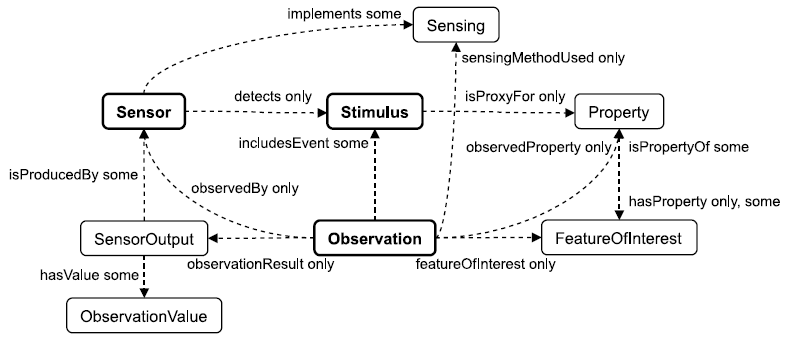
\includegraphics[width=1\linewidth]{figs/sens_stim_obs.png}
	\caption{The stimulus–sensor–observation pattern \cite[p. 28]{SSW:SSN_incubatorGroup}}
	\label{fig:sens-stim-obs}
\end{figure}

\paragraph{Observation capability metadata model} \mbox{}\\
\cite{SW:Hu} have reviewed a number of metadata models (including \ac{sensorml} and \ac{ssno}) for the use of earth observation (including remote sensing). They argue that all of the current metadata models are not sufficient for sensor data discovery. This conclusion is based on an evaluation of six criteria. Three steps have been identified in the process of obtaining relevant sensor data for earth observation, which have been used to derive criteria for their evaluation framework. These steps are sensor filtration, sensor optimisation and sensor dispatch. The filtration of sensors should result in a set of sensors that meets the requirements of the application: it should measure the right phenomenon, be active, be inside the spatial and temporal range, and have a certain sample interval. In sensor optimisation the selected sensors should be combined to complement or enhance each other. To do this, the observation quality, coverage and application is relevant. In the last step - sensor dispatch - the data should be retrieved, stored and transmitted. In every evaluated model the same sensors can be describe in different ways or only partially, which affects the outcome of the sensor dispatch. 

Therefore, a metadata model is proposed that "reuses and extends the existing sensor observation-related metadata standards" \cite[p. 10546]{SW:Hu}. It is composed of five modules: observation breadth, observation depth, observation frequency, observation quality and observation data. They should be derived from metadata elements described using the Dublin Core metadata element set. These five modules can then be formalised following the \ac{sensorml} schema which can be queried by users via a 'Unified Sensor Capability Description Model-based Engine'. 

\paragraph{Om-lite \& sam-lite ontologies} \mbox{}\\
\cite{SSW:Cox4} has been working on a new semantic ontology based on \ac{om}. Previous efforts, such as the \ac{ssno} have been using pre-existing ontologies and frameworks. However, there are already many linked data ontologies that could be useful for describing observation metadata, such as space and time concepts. Also, the \ac{ssno} does not take sampling features into account. Therefore, \cite{SSW:Cox4} proposes two new ontologies: \ac{owl} for observations or om-lite \citep{SSW:Cox3} and \ac{owl} for sampling features or sam-lite \citep{SSW:Cox2}. The om-lite ontology defines the concepts from \ac{om} regarding observations, while the sam-lite defines the sampling feature concepts. A mapping of the \ac{ssno} to om-lite is also provided.

\cite{SSW:Cox4} describes how the PROV ontology \citep{LD:PROV} can be directly used inside om-lite. The PROV ontology is "concerned with the production and transformation of Entities through time-bounded Activities, under the influence or control of Agents" \cite[p. 12]{SSW:Cox4}. This is a very convenient ontology for modelling real world entities, such as sensors, observation processes and sampling processes. Many other ontologies could be implemented in combination with om-lite and sam-lite, depending on the kind of observations that are being modelled and the data publisher's preference. 
 
\subsection{Sensor data aggregation}
Sensor data aggregation can be performed for two purposes: to reduce the energy constraint of sensor networks \citep{SW:Korteweg} or to sample a feature-of-interest in space and/or time \citep{SDI:INSPIRE2}. Sampling is performed when a feature-of-interest is not accessible, in which case "observations are made on a subset of the complete feature, with the intention that the sample represents the whole" \citep{SSW:Cox3}. \cite{SSW:Stasch3} proposes a \ac{wps} that retrieves sensor data from a \ac{sos} service in order to aggregate it based on features-of-interest. The approach by \cite{SSW:Stasch} is similar, but takes sensor data as input that is already published on the semantic web.

\cite{SW:Ganesan} stresses that spatio-temporal irregularities are fundamental to sensor networks. Irregular sampling can have a potentially large influence on the accuracy of the aggregated outcome. For example, averaging sensor data from a feature-of-interest that is being sampled densely in some parts and more sparsely in other parts could lead to inaccurate results. To counter this the values of the densely sampled area should have a lower weight than the values from the sparsely sampled area. The same holds true for temporal irregularities \citep{SW:Ganesan}. Also, \cite{SSW:Stasch4} argue that in order for automatic aggregation to work there needs to be semantics on which kind of aggregation methods are appropriate for a specific kind of sensor data. Not all kinds of aggregation are meaningful (e.g. taking the sum of temperature values). This requires a formalisation of expert knowledge which they call semantic reference systems. 

\subsection{Discussion}
\ac{semsos} \citep{SSW:Henson, SSW:Pschorr} as well as \ac{sel} \citep{SSW:Janowicz} focus on combining the sensor web with the semantic web, but do not address the integration and aggregation of sensor data. Similarly, \cite{SSW:Atkinson} proposes to expose sensor data to the semantic web in order to find other kinds of related data about the same feature-of-interest. Data that can be collected from another area of research. However, \cite{SSW:Atkinson} do not mention the integration of sensor data from heterogeneous sources either. \cite{SSW:Stasch} and \cite{SSW:Stasch3} suggest interesting methods for aggregating sensor data based on features-of-interest. However, also these studies use sensor data from only a single source into account. Moreover, \cite{SSW:Corcho} and \cite{SSW:Ji} argue that methods for integration and fusion of sensor data on the semantic web is still an area for future research. Data fusion is "a data processing technique that associates, combines, aggregates, and integrates data from different sources" \cite[p. 2]{SSW:Wang2}. 

\cite{SW:OGC3} and \cite{SW:OGC4} present methods for including \ac{sos} services in an \ac{ogc} catalogue service using \ac{sor} and \ac{sir}. Making sensor metadata available in a catalogue service will improve the discovery. However, discovery through the semantic web is likely to be more effective, since links can be created towards the sensor data from many different sources of related information. Another advantage is that links can be created by everybody that publishes linked data on the web, allowing sensor data to be used for implementations that were not identified beforehand by the publisher. Also, the semantic web will be easier to access, while the catalogue service can only be accessed at a certain \ac{url} which has to be known to potential users. This thesis therefore focuses on the discovery, integration and aggregation of sensor data using the semantic web.

When publishing data on the semantic web, ontologies are required to specify what things are and how they relate to other things. The evaluation of observation metadata ontologies by \cite{SW:Hu} is interesting, since it exposes what the relevant aspects are in the process of observation discovery. However, its proposed model focusses mainly on including remote sensing and imagery data in metadata models that were not originally created for this kind of data. The \ac{ssno} is an ontology that clearly describes the process between sensor, stimulus and observation. However, \cite{SSW:Cox4} points out that an important aspect of describing a sensor network is missing in this ontology: the sampling. Also, the om-lite and sam-lite ontologies by \cite{SSW:Cox4} are lightweight ontologies that can be complemented by already existing linked data ontologies. They don't rely on the (heavy) \ac{iso} specifications that date from before the semantic web, unlike the \ac{ssno}. The om-lite and sam-lite ontologies will therefore be used in this thesis.  

The idea by \cite{SW:Jones} of delivering data to users through a service with which they are already familiar is very appealing, because it enables data to be immediately used in any existing \ac{gis}. This is also suggested by \cite{SSW:Atkinson} to ease the transition to the linked data world. However, current research has mainly been concerned with static geographic data, not with sensor data. Therefore, this thesis aims to provide a service for integrating and aggregating sensor data as a \ac{wps}.

%!TEX root = ../thesis.tex

\chapter{Research Objectives}
\label{chap:objectives}

the research objectives and/or research questions are clearly defined, along with the scope (ie what you will not be doing);

\section{Research Question} 
How can the Semantic Sensor Web improve the discovery, integration and aggregation of sensor data?



\section{Objective} 
Develop a method to semantically link sensor metadata to real world objects for spatial, semantic and temporal data aggregation.


\section{Scope} 
focus on \ac{ogc}'s \ac{swe} standards / \ac{sos} and \ac{w3c}'s \ac{ssn} ontology. Not going into evaluation of different standards. Not specifically focussing on smart devices.
%!TEX root = thesis.tex
\chapter{Methods}
\label{chap:methods}

overview of the methodology to be used;

\section{Standards}
\subsection{Sensor Web Enablement}
\ac{sos} and \ac{ssn}

\subsection{Semantic Web}

\begin{itemize}
	\item Store \ac{osm} data: create \ac{rdf} on-the-fly to prevent double storage. 
	\item Retrieve sensor metadata: create \ac{rdf} from \ac{om} which is returned by \ac{sos} getCapabilities/describeSensor requests
	\item Use \ac{ssn} as ontology for semantic sensor metadata
	\item Use \ac{owl} as language for storing semantic \ac{rdf} triples
\end{itemize}


Query metadata: SPARQL, geo-SPARQL or stSPARQL? and which query engine?

\section{Ontologies}
The \ac{om} ontology is retrieved from sensors\\
Use \ac{ssn} ontology ontology to store metadata from sensors.  

\section{Middleware}
Creating own middleware to link sensors semantically and retrieve aggregated data\\

\ac{rest}ful service





%!TEX root = thesis.tex

%time planning—having a Gantt chart is probably a better idea then just a list;

\chapter{Planning}
\label{chap:planning}

This chapter provides an overview of the deadlines for the thesis, ranging from the start of the thesis on November tenth, 2015 to the final deadline on June twentieth, 2016. Based on these deadlines a planning has been made, which breaks down the total workload into twelve parts. A GANTT chart is presented as a graphical presentation of the thesis planning. 

\section{Deadlines}
For the planning of the thesis a number of deadlines are import. At five moments in time the status of the thesis has to be presented and at three of these moments it is required to hand in a report. The five deadlines are referred to as P1 to P5 in the graduation manual. P1 took place on November tenth, 2015. The general idea for the thesis was presented here and a number of students and staff was present to provide feedback. This document is part of the deliverables for P2. At P2 the research proposal for the thesis needs to be handed in. This contains the research question, its relevance, a literature analysis of related work, a description of the methods, a planning and an overview of the tools and data that will be used. The research proposal is due January eleventh, 2016. The P2 presentation is scheduled on January eighteenth, 2016. Preliminary results are presented at P3, for which the date is still unknown. The P4 deadline is on May second, 2016. This is the deadline for handing in the first draft of the thesis report. It should also be presented on May seventh, 2016. The final deadline (P5) is on the thirteenth of June, 2016. The thesis outcomes will be presented on June twentieth, 2016.

\section{GANTT Chart}
\begin{figure}
	\centering
	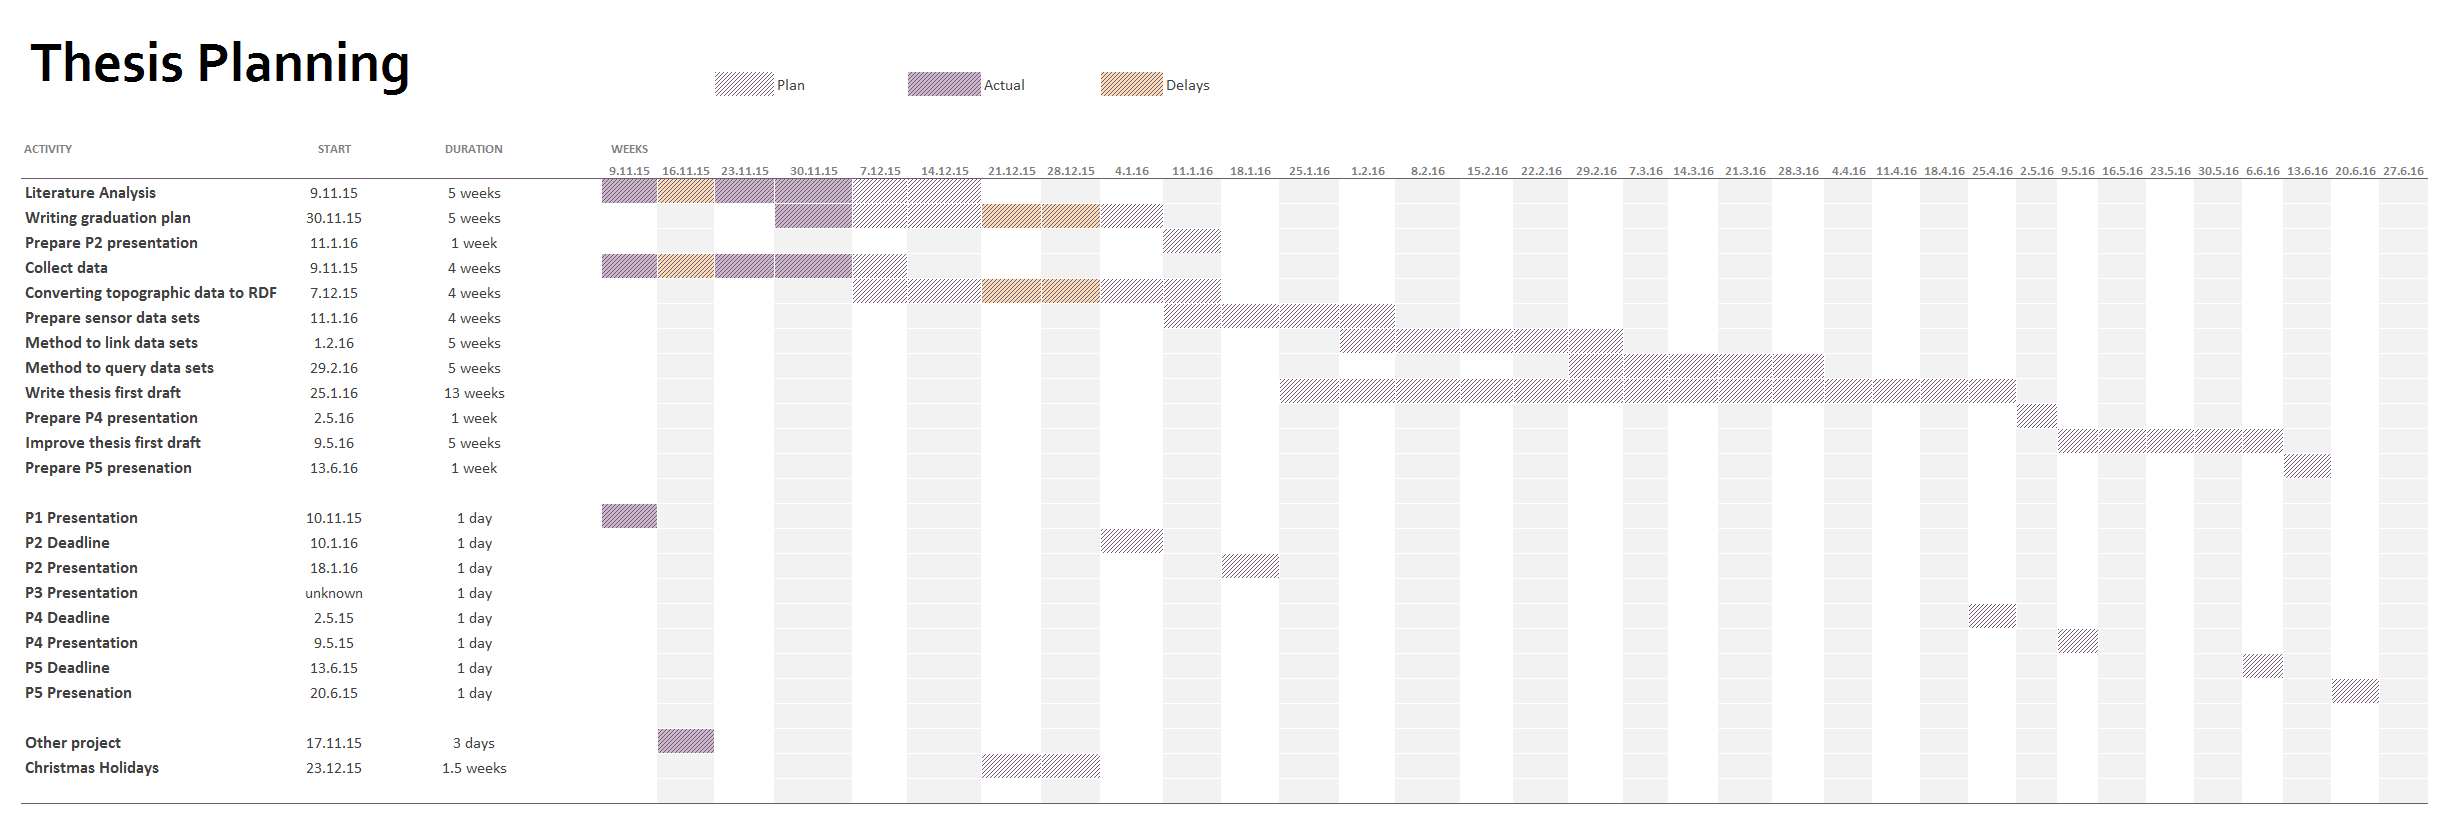
\includegraphics[width=2\linewidth, angle=90]{figs/GANTT-chart.png}
	\caption{GANTT chart showing the planning of the thesis}
	\label{fig:GANTT}
\end{figure}
%!TEX root = thesis.tex
\chapter{Tools and Data}
\label{chap:TD}

since specific data and tools have to be used, it’s good to present these concretely, so that the mentors know that you have a grasp of all aspects of the project;

\section{Data}
Topographic data of neighbourhoods, city districts, municipalities and provinces\\
Air quality sensor data from the \ac{rivm} (\url{http://inspire.rivm.nl/sos/}) and from the \ac{ircel} (\url{http://sos.irceline.be/}).

\section{Database}
A Postgres database will be used with the Postgis extension.

\section{Server}
Prototyping will be done using a localhost at first, but in the end it could be hosted on the university server.

\section{Prototype}
\begin{itemize}
	\item The Python programming language will be used for scripting a prototype. 
	\item Psycopg2 will be used to connect a Python script to a Postgres database.
	\item Python's \href{http://docs.python-requests.org/en/latest/user/quickstart/}{Request} library will be used for making \ac{http} POST and GET requests. 
	\item For working with \ac{xml} Python's xml package will be used.
	\item To create \ac{rdf} documents the Python library RDFLib will be used. 
\end{itemize}









  



% *****************************************************************
% Backmatter
%******************************************************************
\appendix

%%%
%- bibliography
\clearpage
\bibliographystyle{apalike}
\bibliography{Thesis_sources}


\end{document}





